% =====================================================================
%  Partie 1 — Contexte environnemental
%  Les figures des diapositives sont signalées en commentaire « FIGURE ».
% =====================================================================
\part{Contexte environnemental}

Cette partie présente les notions d'enjeux environnementaux, la place du secteur du bâtiment dans ces enjeux, puis le cadre réglementaire qui impose aujourd'hui l'ACV dans la construction neuve en France : la RE 2020.

% ---------------------------------------------------------------------
\chapter{Enjeux environnementaux}

 
Lorsqu'on parle d'enjeux environnementaux, on pense en premier lieu au climat, qui n'est pourtant que l'une de leurs trois composantes que voici :
 
\begin{itemize}
    \item \textbf{le climat} : la succession des conditions météorologiques de la planète (température, humidité et pression de l'atmosphère) sur de longues périodes temporelles (à ne pas confondre avec la météo qui est sur le temps court : « quel temps fera-t-il demain ? »)
    \item \textbf{les ressources} : les stocks d'eau ou de
    ressources minérales et fossiles
    \item \textbf{la santé} : à la fois humaine
    (pollution de l'air, îlots de chaleur, etc.) et celle des écosystèmes (biodiversité, sols, milieux aquatiques)
\end{itemize}
 
Le secteur du bâtiment intervient sur ces trois plans : il émet des gaz à effet de serre, de la construction comme à l'usage, il consomme de grandes quantités de matières premières en impactant ses écosystèmes, et il conditionne le confort et la santé des usagers.

\paragraph{L'ère de l'Anthropocène}
Le terme \emph{Anthropocène} désigne une période au cours de laquelle les activités humaines sont devenues une force capable de modifier le fonctionnement du système terrestre dans son ensemble.
 
Les travaux de Steffen\footfullcite{steffen_trajectory_2015} illustrent ce basculement en suivant, de 1750 à 2010, deux séries d'indicateurs. Les premiers décrivent le développement socio-économique
mondial : population, PIB, consommation d'énergie primaire, d'eau, d'engrais, urbanisation, transports, etc., voir figure~\ref{fig:anthropocene1}. Les seconds décrivent l'état du système terrestre : concentrations en gaz à effet de serre, acidification des océans, température de surface, perte de forêts tropicales, dégradation de la biosphère, etc., voir figure~\ref{fig:anthropocene2}.
 
\begin{figure}[htbp]
    \centering
    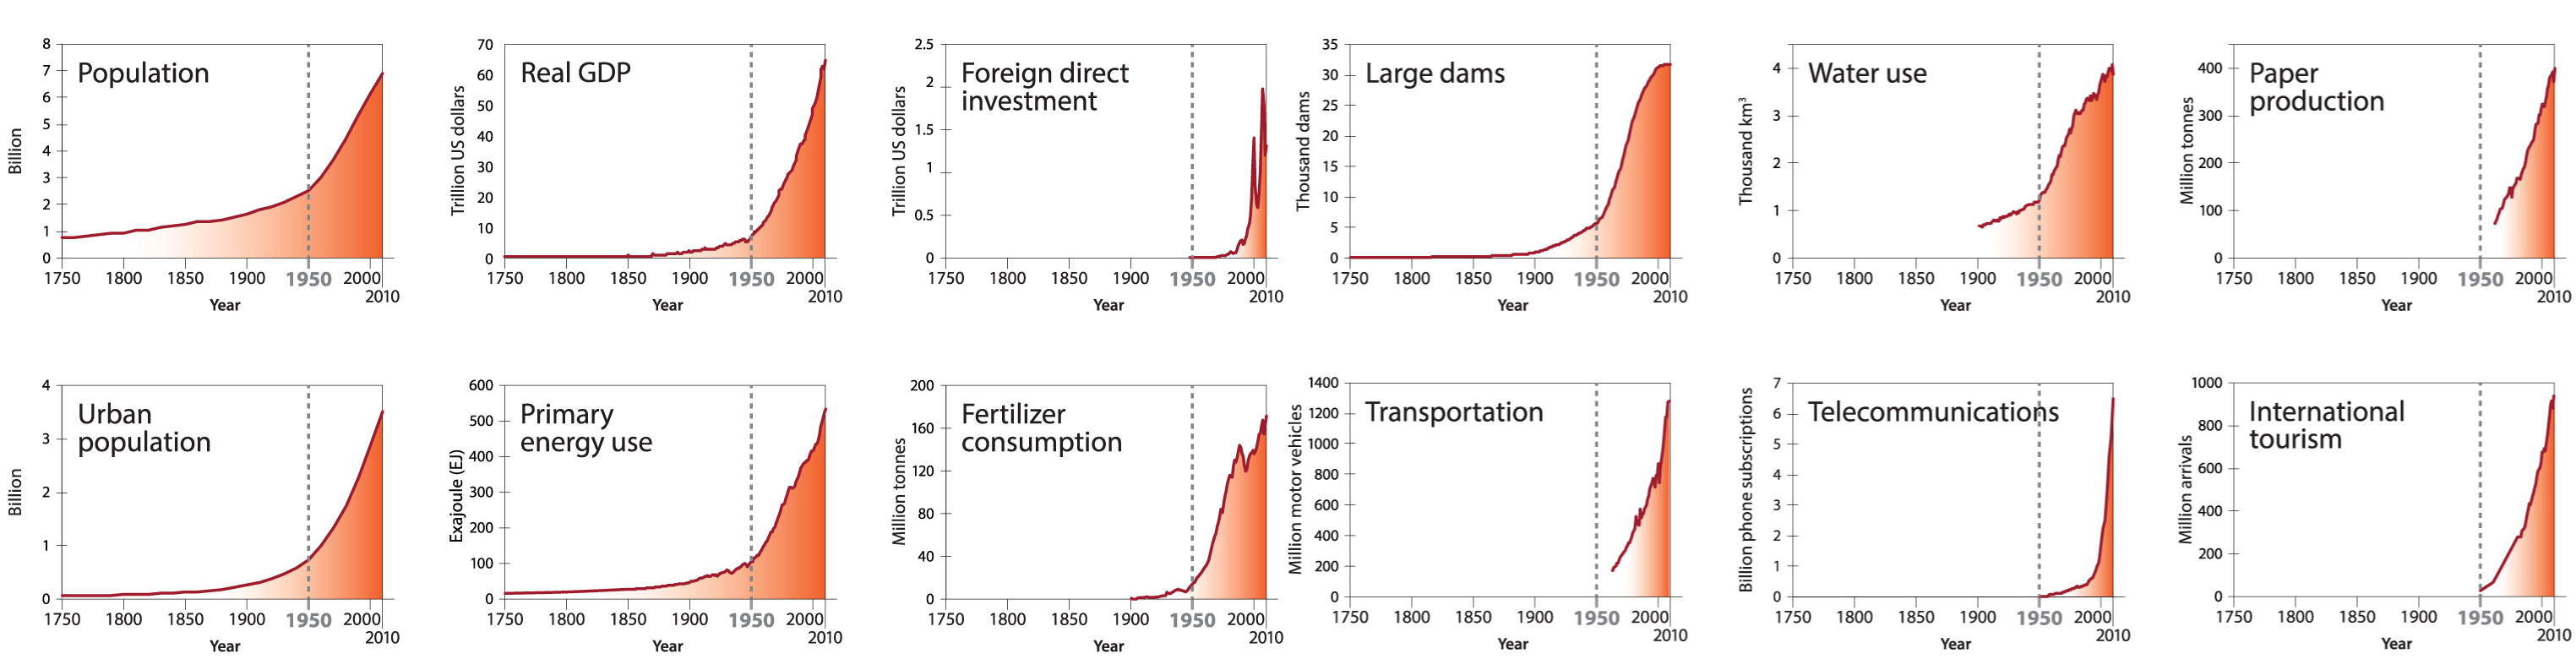
\includegraphics[width=\linewidth]{figures/Anthropocene1V.jpg}
    \caption{Évolution, de 1750 à 2010, de différents indicateurs mondiaux
    du développement socio-économique.}
    \label{fig:anthropocene1}
\end{figure}
 
\begin{figure}[htbp]
    \centering
    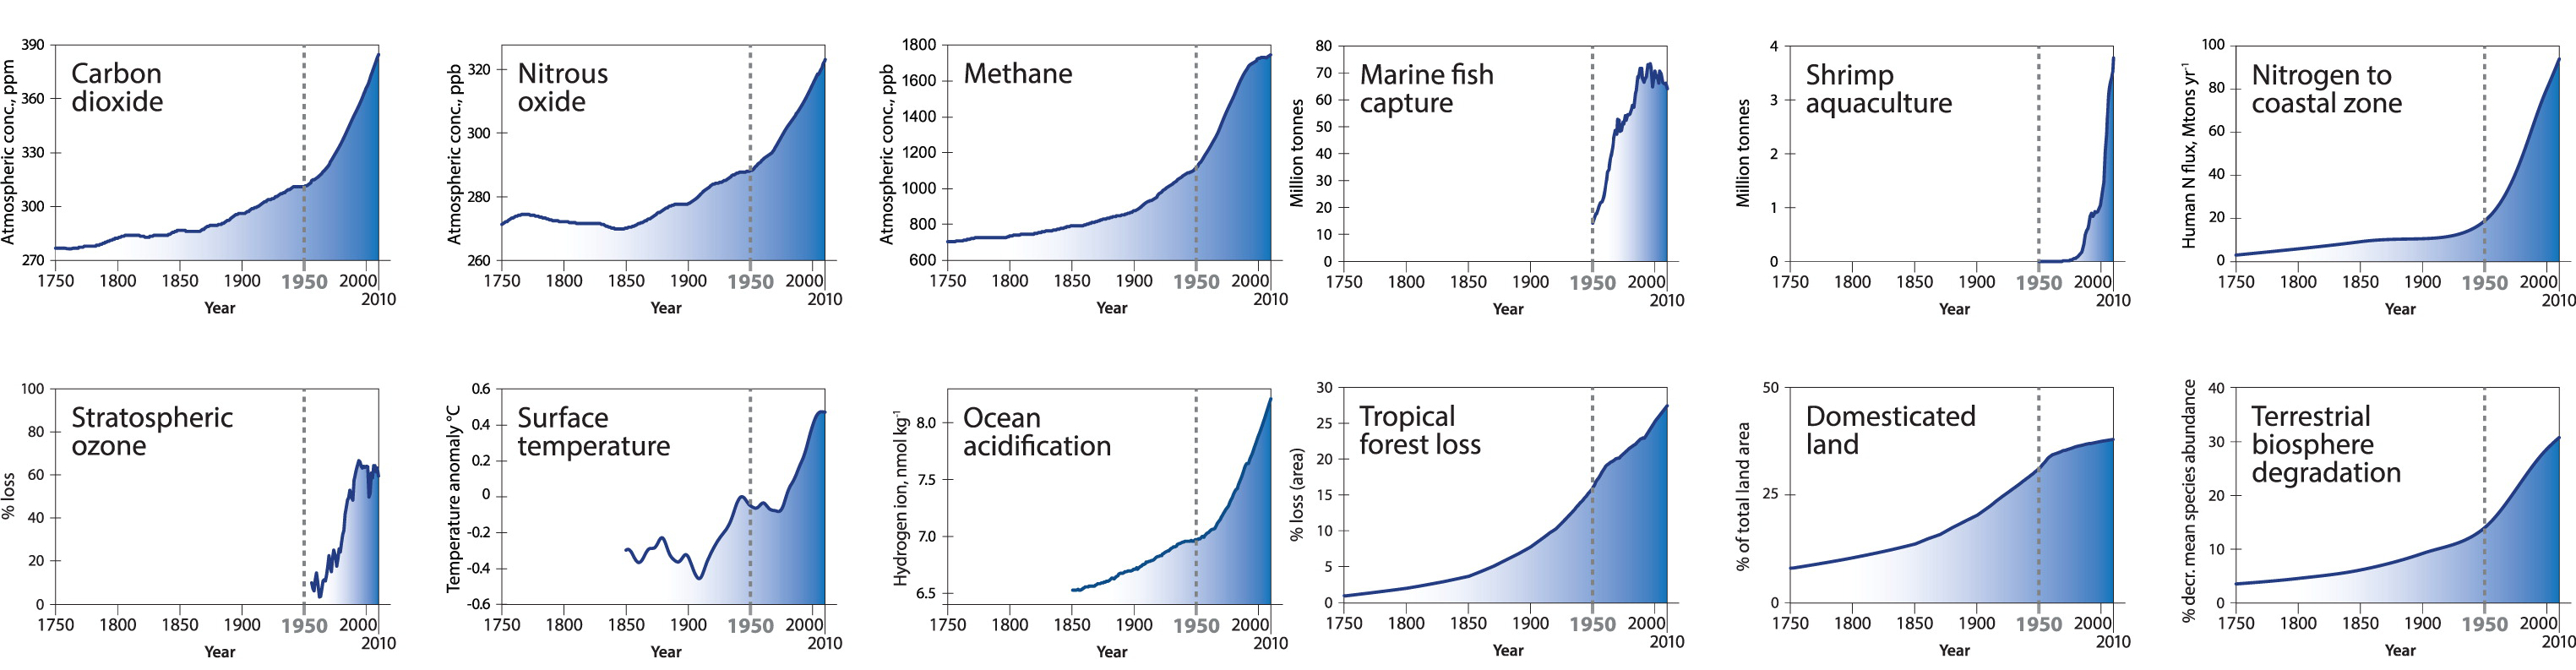
\includegraphics[width=\linewidth]{figures/Anthropocene2V.jpg}
    \caption{Évolution, de 1750 à 2010, de différents indicateurs du
    système terrestre.}
    \label{fig:anthropocene2}
\end{figure}
 
Ces deux séries présentent la même allure : une évolution lente jusqu'au milieu du \textsc{xx}\textsuperscript{e}~siècle, puis une envolée à partir des années 1950. Cette simultanéité, que les auteurs nomment la \emph{Grande Accélération}, met en évidence le lien direct entre la croissance des activités humaines et la dégradation du système terrestre.

\section{Climat}
\subsection*{L'effet de serre}
\label{chap:effet-serre}

\subsubsection*{Mécanisme de l'effet de serre}
Le mécanisme de l'effet de serre peut se décomposer en plusieurs étapes\footfullcite{oce}$^,$\footfullcite{reveilleur-effet-serre}$^,$\footfullcite{ipcc_climate_2021} et est illustré dans la figure~\ref{fig:serre}.
\begin{enumerate}
  \item \textbf{Rayonnement venant du Soleil} : le rayonnement solaire atteint le haut de l'atmosphère.
  \item \textbf{Traversée de l'atmosphère terrestre} : une partie du rayonnement est réfléchie vers l'espace, une autre est transmise vers la surface de la Terre.
  \item \textbf{Arrivée à la surface de la Terre} : une partie du rayonnement est réfléchie vers l'atmosphère, l'autre est absorbée par la surface.
  \item \textbf{Accumulation d'énergie} : la température de la surface terrestre augmente car elle reçoit l'énergie du Soleil.
  \item \textbf{Émission de rayonnement infrarouge} : tous les corps émettent du rayonnement en fonction de leur température\footfullcite{stefan1879}. Les objets chauds rayonnent davantage que les objets froids. La surface de la Terre émet alors un rayonnement infrarouge, qui transporte de la chaleur vers l'atmosphère.
  \item \textbf{Effet de serre} : certains gaz de l'atmosphère absorbent une partie du rayonnement infrarouge, empêchant toute la chaleur de ce rayonnement de s'échapper dans l'espace. Ces gaz chauffent et réémetten de l'infrarouge.
  \item \textbf{Nouvelle absorption par la surface} : la surface de la Terre se réchauffe alors davantage.
\end{enumerate}

\begin{figure}[h]
    \centering
    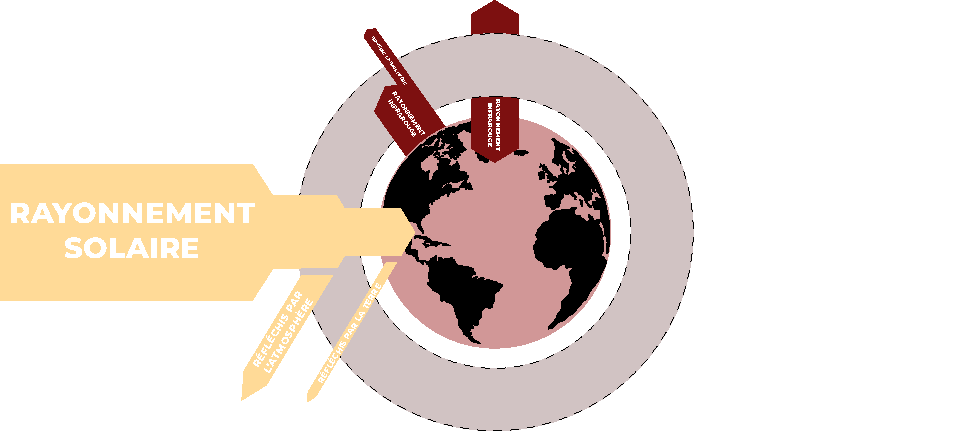
\includegraphics[width=1\linewidth]{figures/serre.pdf}
    \caption{Schéma de principe de l'effet de serre}
    \label{fig:serre}
\end{figure}

La Terre, plus froide que le Soleil, rayonne dans l'infrarouge. Sans effet de serre, la température de la Terre serait à l'équilibre autour de $-18$\,°C. Avec l'effet de serre, la température de la Terre s'équilibre autour de 15\,°C.

Ainsi, l'effet de serre n'est ni « bon » ni « mauvais » : c'est un mécanisme naturel qui maintient la température moyenne de la surface de la Terre. Le principal gaz à effet de serre est la vapeur d'eau. Sa quantité dans l'atmosphère est globalement stable depuis des milliers d'années\footnote{La quantité de vapeur d'eau dans l'air dépend de la température : si l'atmosphère se réchauffe, elle pourra contenir plus de vapeur d'eau avant saturation. Avec le réchauffement climatique, la quantité de vapeur d'eau a tendance à augmenter et donc à amplifier davantage le phénomène de réchauffement.}. La partie suivante montre l'impact de l'être humain sur l'augmentation de la quantité de gaz à effet de serre dans l'atmosphère. C'est cette augmentation de gaz à effet de serre qui augmente le forçage radiatif conduisant la Terre à se réchauffer.

Les gaz à effet de serre sont simplement définis comme les gaz absorbant le rayonnement infrarouge, c'est une propriété intrinsèque à chaque gaz (certains absorbent le rayonnement infrarouge, d'autres non).

\subsubsection*{Limite de l'analogie}
L'effet de serre n'est toutefois pas analogue au fonctionnement d'une serre agricole. Dans une serre agricole fermée, le réchauffement de l'air est issu du rayonnement solaire (qui chauffe le sol) mais surtout de la convection : dans une serre fermée, l'air chaud ne peut pas s'échapper et reste dans la serre.

Ce n'est donc pas la même chose que l'effet de serre, qui est l'émission de rayonnement infrarouge par la Terre, rayonnement qui est absorbé par les gaz à effet de serre contenus dans l'atmosphère. Ce rayonnement absorbé réchauffe l'atmosphère qui, étant plus chaude, rayonne également de l'infrarouge vers l'espace et vers la Terre, conduisant à son réchauffement.

\subsection*{Évolution et contribution anthropique}
La figure~\ref{fig:GES}, issue du GIEC\footfullcite{ipcc_climate_2022}, illustre l'évolution des gaz à effet de serre, cette évolution est due aux différentes activités humaines. Le Secten, réalisé par le Citepa\footfullcite{citepa_secten_2024}, illustre la répartition des GES en France par secteur (figure~\ref{fig:GES2}).
\begin{figure}
    \centering
    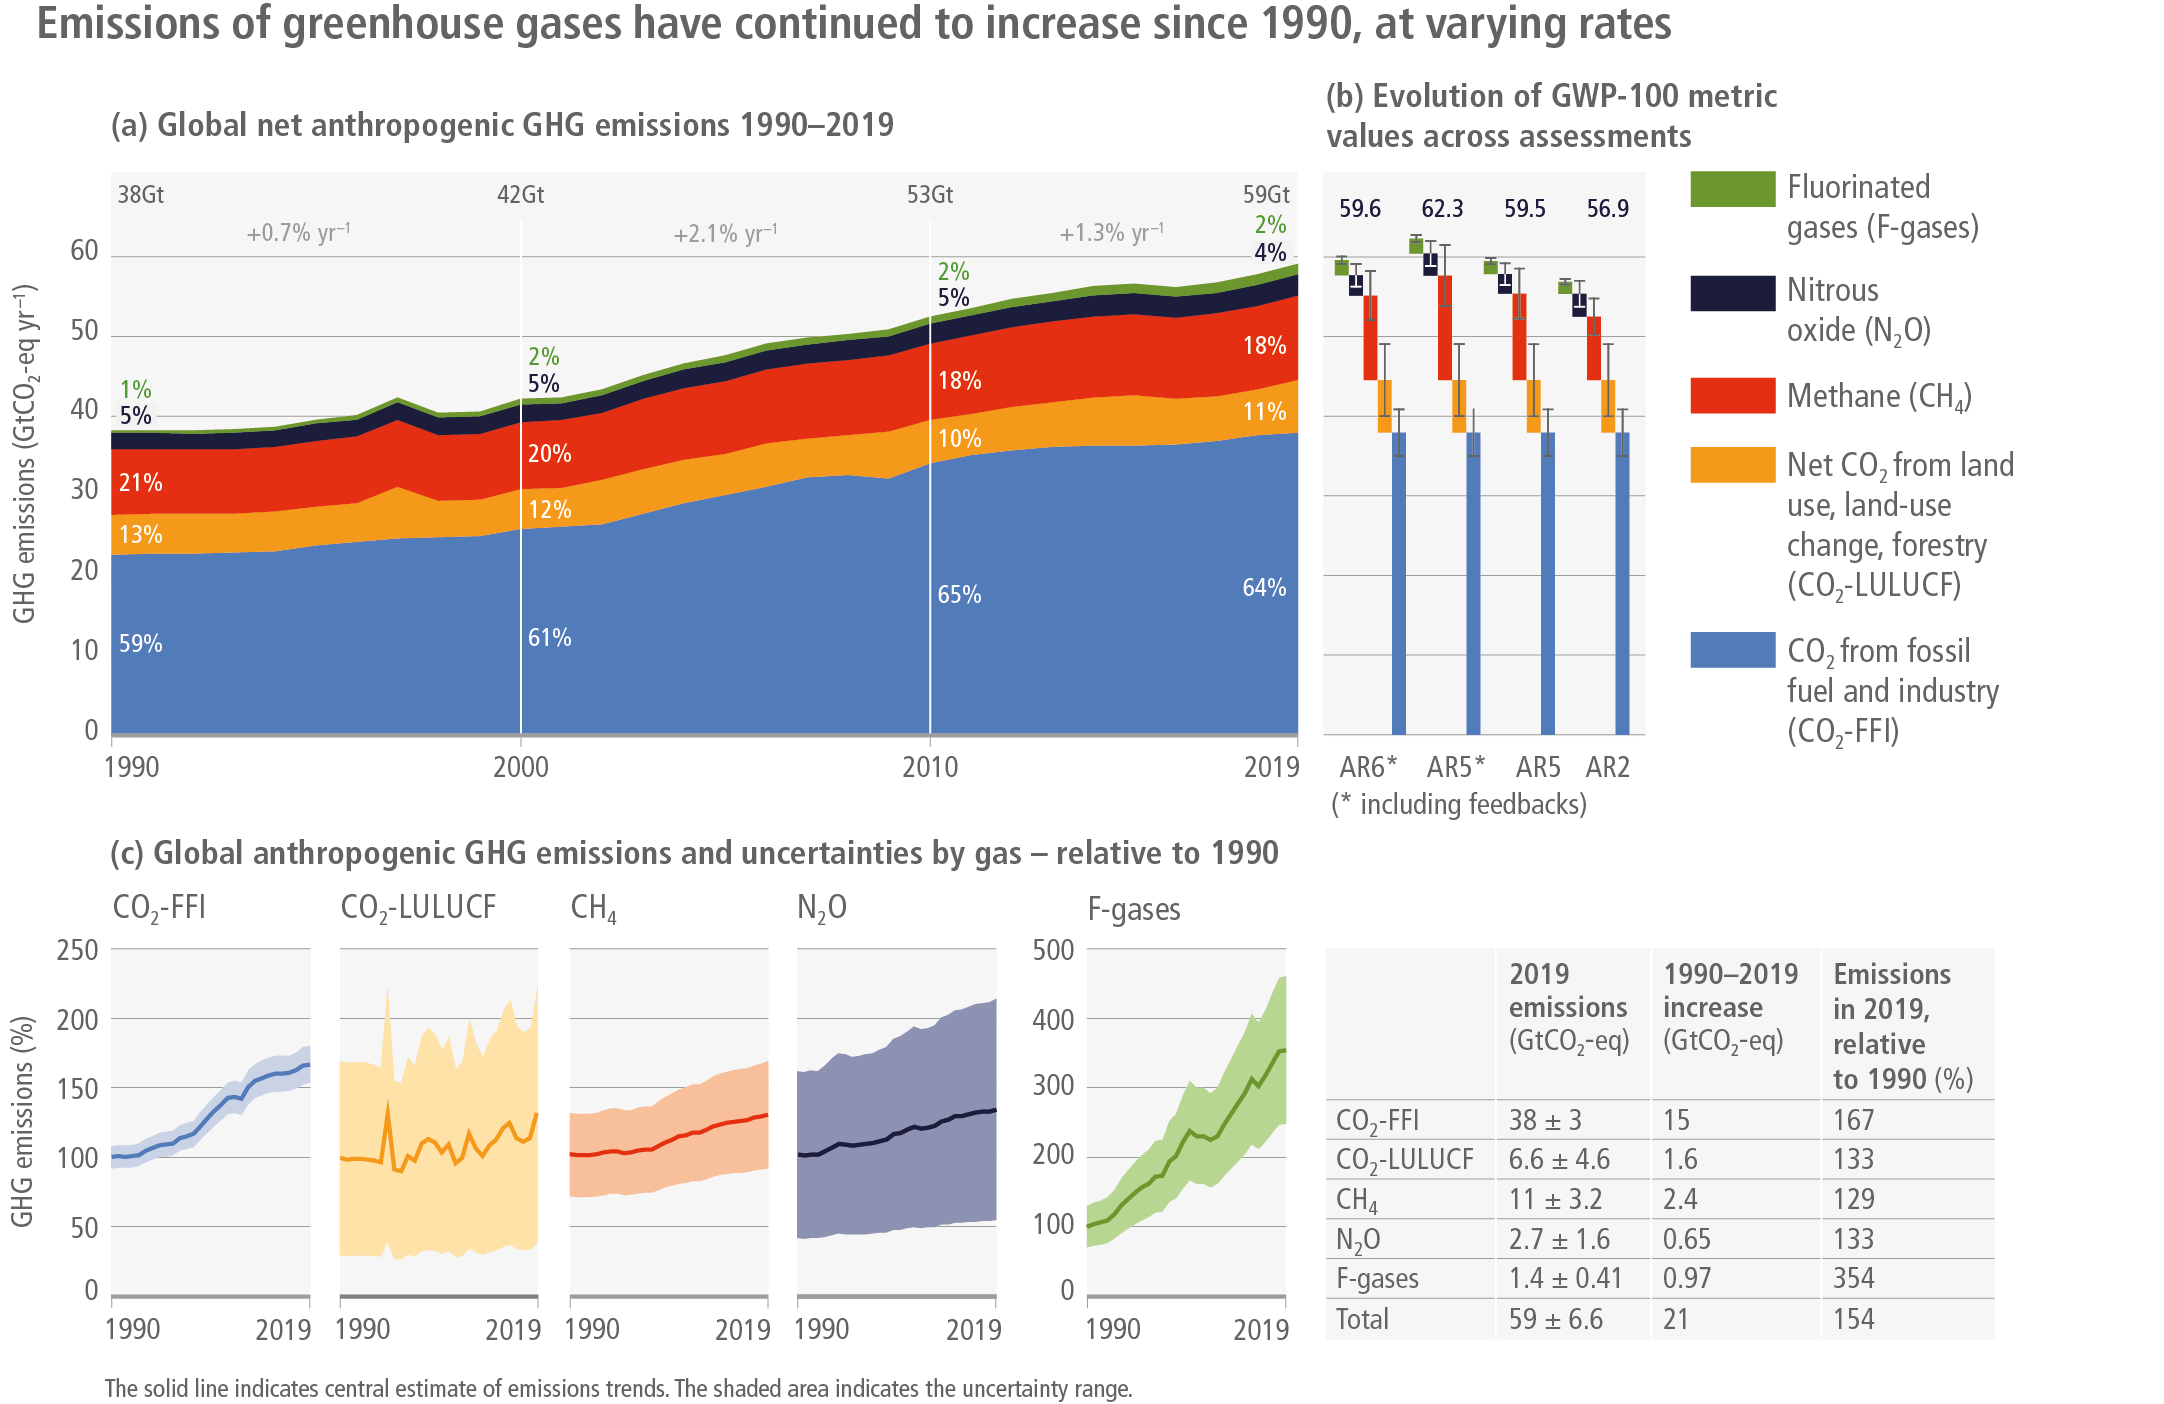
\includegraphics[width=1\linewidth]{figures/GES evolution.png}
    \caption{Évolution anthropique des GES\cite{ipcc_climate_2022}}
    \label{fig:GES}
\end{figure}

\begin{figure}
    \centering
    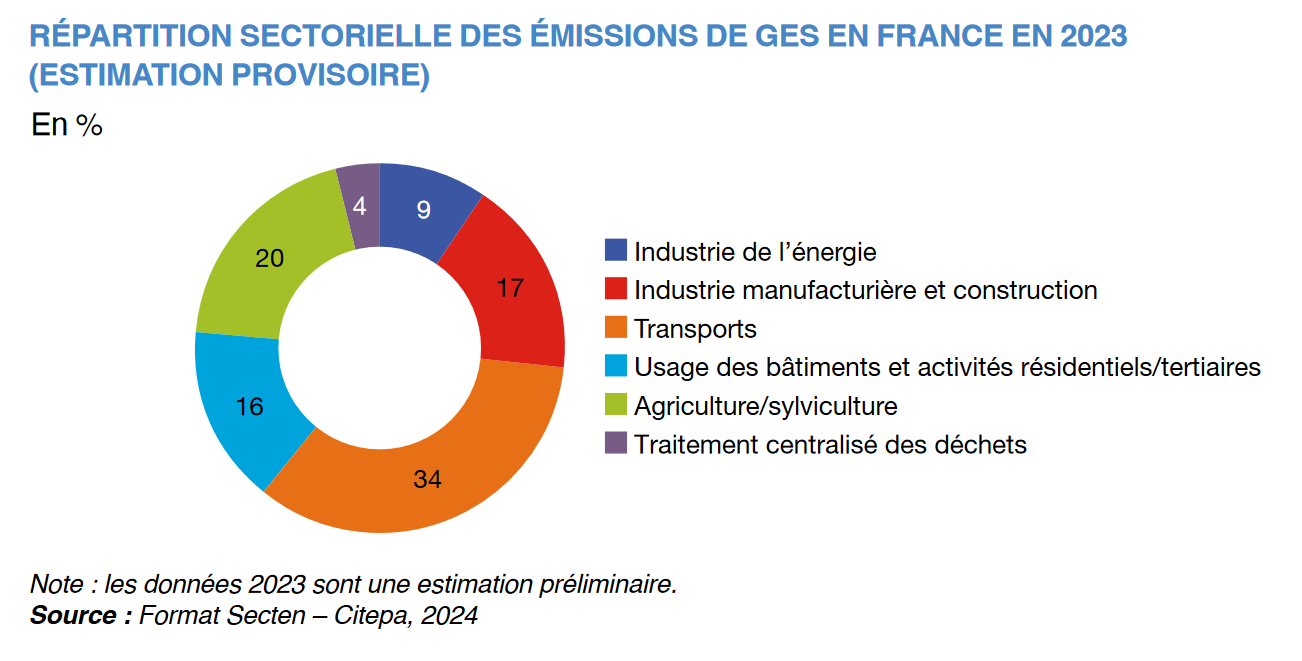
\includegraphics[width=1\linewidth]{figures/ADEME.png}
    \caption{Contribution des GES par secteur en France}
    \label{fig:GES2}
\end{figure}
\subsection*{Atténuation et adaptation face au changement climatique}
On distingue les notions d'atténuation et d’adaptation face au changement climatique (les définitions, différences et rôle en architecture seront détaillés ci-dessous).

\subsubsection*{Atténuation}
Définition (glossaire du GIEC\footfullcite{giec_sr15_glossaire}) : \textit{Intervention humaine visant à réduire les émissions ou à renforcer les puits de gaz à effet de serre.}
\subsubsection*{Adaptation}
Définition (glossaire du GIEC) : \textit{Pour les systèmes humains, démarche d’ajustement au climat actuel ou attendu ainsi qu’à ses conséquences, de manière à en atténuer les effets préjudiciables et à en exploiter les effets bénéfiques. Pour les systèmes naturels, démarche d’ajustement au climat actuel ainsi qu’à ses conséquences. L’intervention humaine peut faciliter l’adaptation au climat attendu et à ses conséquences.}
% TODO : à compléter
\section{Ressources}

Une croissance infinie de la consommation de matières est incompatible avec un monde aux ressources finies. Cette contrainte concerne directement le secteur de la construction, consommateur de granulats, de sable, de métaux et d'énergie fossile\footfullcite{jancovici-blain2021}$^,$\footfullcite{bihouix-perriot2024}.

% FIGURES : Figures/sansfin.jpg et Figures/ressources.jpg

\subsection*{Jour du dépassement}

Le jour du dépassement\footfullcite{gfn-overshootday} compare deux grandeurs\footfullcite{gfn-glossary} :
\begin{itemize}
  \item la \textbf{biocapacité} : la capacité des écosystèmes à fournir des matières biologiques utiles et à assimiler les déchets générés par les êtres humains
  \item l'\textbf{empreinte écologique} : la surface biologiquement productive de terre et d'eau dont un individu, une population humaine ou une activité a besoin pour produire les ressources qu'elle consomme et absorber les déchets qu'elle génère, en utilisant les technologies et les pratiques de gestion des ressources existantes
\end{itemize}

\begin{encadre}{Pour calculer le jour du dépassement}
\begin{itemize}
  \item Individuel : \url{https://www.footprintcalculator.org/fr}
  \item Par pays : \url{https://data.footprintnetwork.org}
\end{itemize}
\end{encadre}

% FIGURE : Figures/Overshoot.png
% FIGURE : Figures/biocapacité.png
%   Biocapacité française

\section{Santé}

La santé concerne à la fois la santé humaine (pollution de l'air, îlots de chaleur, etc.) et celle des écosystèmes (biodiversité, sols, milieux aquatiques). Deux exemples, l'eutrophisation et la formation d'ozone photochimique, sont détaillés avec les indicateurs de l'ACV (partie~3).

% ---------------------------------------------------------------------
\chapter{Impact du secteur du bâtiment}

% FIGURE : Figures/fallingwater.jpg
%   Maison sur la Cascade, Frank Lloyd Wright, 1939. Crédit Britannica
% FIGURE : Figures/fallingwater_R
%   Maison sur la Cascade, chantier de rénovation (2025 ?). Crédit Jason Nark / The Philadelphia Inquirer

\section{Impact du secteur du bâtiment dans le monde}

En 2019, le secteur du bâtiment représente 21\,\% des émissions mondiales de gaz à effet de serre (GES)\footfullcite{ipcc_climate_2022}. Ces émissions se décomposent en :
\begin{itemize}
  \item 57\,\% liées à la production d'électricité et de chaleur (exploitation)
  \item 24\,\% liées à la construction
  \item 18\,\% liées aux matériaux, essentiellement le béton et l'acier
\end{itemize}

Entre 1990 et 2019, les émissions de GES du bâtiment ont augmenté de 50\,\% et sa consommation électrique de 138\,\%.

\section{Impact du secteur du bâtiment en France}

En 2017, le secteur du bâtiment représente 23\,\% des émissions de GES en France\footfullcite{ademe-batiments}. Pour les bâtiments neufs, 70\,\% de ces émissions sont liées à la phase de construction (chantier et matériaux).

Le secteur du bâtiment représente également 45\,\% de la consommation énergétique nationale.

% ---------------------------------------------------------------------
\chapter{Cadre réglementaire, la RE 2020}

\section{Présentation}

La France s'est dotée d'une réglementation environnementale en 2022, qui prend progressivement la suite de la RT 2012 : la RE 2020. Nous passons d'une Réglementation Thermique (RT) à une Réglementation Environnementale (RE).

Elle poursuit des objectifs d'amélioration de la performance énergétique des bâtiments neufs, de réduction de leur impact sur le climat (prise en compte des émissions de gaz à effet de serre sur l'ensemble du cycle de vie des bâtiments) et de leur adaptation aux conditions climatiques futures (renforcement du confort d'été)\footfullcite{guide-re2020}.

\subsection*{Catégories et indicateurs}

La RE 2020 s'articule autour de trois catégories (carbone, énergie, confort d'été) et de six indicateurs (tableau~\ref{tab:re2020-indicateurs}).

\begin{table}[htbp]
\centering
\caption{Les six indicateurs de la RE 2020}

\small
\renewcommand{\arraystretch}{1.25}
\begin{tabular}{p{1.6cm}p{2.6cm}p{3.8cm}p{6cm}}
\textbf{Catégorie} & \textbf{Indicateur} & \textbf{Définition} & \textbf{Description} \\
\hline
Carbone & $I_c$ construction (kgeqCO$_2$/m$^2$) & Impact sur le changement climatique associé aux « composants » et au « chantier » & Utilisation de la méthode d'Analyse de Cycle de Vie pour l'évaluation des émissions de gaz à effet de serre. \\
\cline{2-4}
 & $I_c$ énergie (kgeqCO$_2$/m$^2$) & Impact sur le changement climatique associé aux consommations d'énergie primaire & Utilisation de la méthode d'Analyse de Cycle de Vie pour l'évaluation des émissions de gaz à effet de serre concernant l'énergie consommée pendant le fonctionnement du bâtiment. \\
\hline
Énergie & $C_{ep}$ (kWhep/(m$^2$.an)) & Consommation d'énergie primaire totale & Évaluation de la consommation d'énergie primaire durant la vie du bâtiment. \\
\cline{2-4}
 & $C_{ep,nr}$ (kWhep/(m$^2$.an)) & Consommation d'énergie primaire non renouvelable & Évaluation de la consommation d'énergie non renouvelable durant la vie du bâtiment. \\
\cline{2-4}
 & $B_{bio}$ (points) & Besoins bioclimatiques & Évaluation des besoins de chaud, de froid et d'éclairage. \\
\hline
Confort d'été & DH (°C.h) & Degrés-heures d'inconfort : niveau d'inconfort perçu par les occupants sur l'ensemble de la saison chaude & Évaluation des écarts entre la température du bâtiment et la température de confort. \\
\hline
\end{tabular}
\label{tab:re2020-indicateurs}
\end{table}


\subsection*{Progressivité}

La RE 2020 est entrée en vigueur le 1\textsuperscript{er} janvier 2022 pour les maisons individuelles et les logements collectifs, puis elle a progressivement intégré différents usages. À partir du 1\textsuperscript{er} mai 2026, quasiment tous les programmes de constructions neuves sont concernés. L'application de la RE 2020 aux projets de rénovation n'est actuellement ni prévue ni annoncée, mais cela peut bien entendu évoluer (à suivre).
Pour chaque indicateur, la RE 2020 fixe un seuil à ne pas dépasser. Les seuils carbone et énergie sont renforcés en plusieurs phases : 2025, 2028 puis 2031.

\section{Les indicateurs carbone}

L'ACV est imposée dans le cadre de la RE 2020 pour la catégorie carbone, via les deux indicateurs Ic construction et Ic énergie.

\subsection*{Ic construction}
L'Ic construction (kgeqCO$_2$/m$^2$) représente l'impact de la construction sur le changement climatique. Il prend en compte les matériaux, les équipements ainsi que leur mise en œuvre sur le chantier : un bilan carbone sur les matériaux, les équipements et le chantier est à effectuer en prenant en compte tout le cycle de vie du bâtiment (du transport des matériaux lors de leur fabrication jusqu'à la démolition de l'ouvrage). Les seuils moyens sont évolutifs et donnés par typologie de programme dans le tableau~\ref{tab:ic-construction}.

\begin{table}[h]
\centering
\caption{Seuils Ic\,construction,maxmoyen (kgCO$_2$e/m$^2$)}
\label{tab:ic-construction}
\begin{tabular}{lcccc}
\hline
Usage & 2022 & 2025 & 2028 & 2031 \\
\hline
Logement & 740 & 650 & 580 & 490 \\
Bureau & 980 & 810 & 710 & 600 \\
Enseignement & 900 & 770 & 680 & 590 \\
\hline
\end{tabular}
\end{table}

\subsection*{Ic énergie}
L'Ic énergie (kgeqCO$_2$/m$^2$) représente l'impact de l'énergie sur le changement climatique (il prend en compte la consommation d'énergie et d'eau). Un bilan carbone est à effectuer en prenant en compte l'impact carbone de la production d'énergie et d'eau utilisées dans le bâtiment durant toute sa durée de vie. Les seuils moyens sont donnés dans le tableau~\ref{tab:ic-energie}.

\begin{table}[h]
\centering
\caption{Seuils Ic\,énergie,maxmoyen (kgCO$_2$e/m$^2$)}
\label{tab:ic-energie}
\begin{tabular}{lccc}
\hline
Usage & 2022 & 2025 & 2028 \\
\hline
Logement & 560 & 320 & 260 \\
Bureau & 280 & 200 & -- \\
Enseignement primaire et secondaire & 240 & 200 & 140 \\
\hline
\end{tabular}
\end{table}

Le calcul de ces deux indicateurs repose sur une ACV dynamique, présentée dans la partie~4.

\section{Énergie}

\subsection*{Énergie primaire} L'énergie primaire est une forme d'énergie disponible dans la nature avant toute transformation\footfullcite{sdes-energie}\footnote{\texttt{https://www.statistiques.developpement-durable.gouv.fr/}}. L'évolution de la consommation d’énergie primaire de la France est présentée sur la figure~\ref{fig:primaire} et sa répartition est détaillée ci-dessous :
\begin{itemize}
  \item 43\,\% de nucléaire
  \item 26\,\% de pétrole
  \item 12\,\% de gaz naturel
  \item 16\,\% d'énergies renouvelables et déchets (dont 1\,\% de déchets non renouvelables)
  \item 2\,\% de charbon
\end{itemize}


\begin{figure}
    \centering
    \includesvg[width=0.5\linewidth]{figures/primaire.svg}
    \caption{Évolution de la consommation d’énergie primaire française}
    \label{fig:primaire}
\end{figure}

\subsection*{Consommation d'énergie primaire}
La consommation d'énergie primaire $C_{ep}$ (kWhep/(m$^2$.an)) est estimée pour le bâtiment et doit être inférieure à certains seuils, voir tableau~\ref{tab:cep-seuils}.

\subsection*{Consommation d'énergie primaire non renouvelable}
De même, la consommation d'énergie primaire non renouvelable $C_{ep,nr}$ (kWhep/(m$^2$.an)) doit être inférieure à un certain seuil. La RE 2020 distingue le $C_{ep}$ du $C_{ep,nr}$ pour favoriser l'utilisation d'énergie renouvelable, et assurer des bâtiments plus sobres en consommation d'énergie (ce n'est pas parce que l'énergie est renouvelable que l'on veut la gaspiller).

\begin{table}[htbp]
\centering
\caption{Seuils de consommation d'énergie primaire (kWhep/(m$^2$.an))}
\label{tab:cep-seuils}
\begin{tabular}{l|c|c}

\textbf{Usage} & \textbf{$C_{ep,\mathrm{maxmoyen}}$} & \textbf{$C_{ep,nr,\mathrm{maxmoyen}}$} \\
\hline
Logement collectif & 85 & 70 \\
Bureau & 85 & 75 \\
Enseignement primaire & 72 & 65 \\

\end{tabular}
\end{table}

\subsection*{Besoin bioclimatique}
Le calcul du $B_{bio}$ RE 2020 comprend les besoins en chauffage, en refroidissement et en éclairage du bâtiment.
Le $B_{bio}$ s'intéresse au bâti sans ses équipements.

Le $B_{bio}$ s'intéresse à :
\begin{itemize}
  \item l'orientation
  \item l'isolation
  \item la compacité
  \item les surfaces vitrées
  \item la protection solaire
  \item l'inertie
  \item la conception globale de l'enveloppe
\end{itemize}

Le $B_{bio}$ est une note en points, calculée pendant la conception du bâtiment.

\section{Confort d'été}
\subsection*{Degrés-heures d'inconfort}

Chaque heure, on compte l'écart entre la température du bâtiment et la température limite de confort.
Le calcul des degrés-heures d'inconfort (DH) suit les étapes suivantes, et est illustré figure~\ref{fig:dh} :

\begin{enumerate}
  \item La température extérieure est estimée à partir de fichiers météo prenant en compte des scénarios caniculaires.
  \item Un calcul de la température du bâtiment est effectué (simulation avec un logiciel spécialisé).
  \item On regarde pour chaque heure si la température du bâtiment dépasse la température de confort, si oui on compte de combien de degrés elle dépasse la température de confort.
\end{enumerate}

\begin{figure}
    \centering
    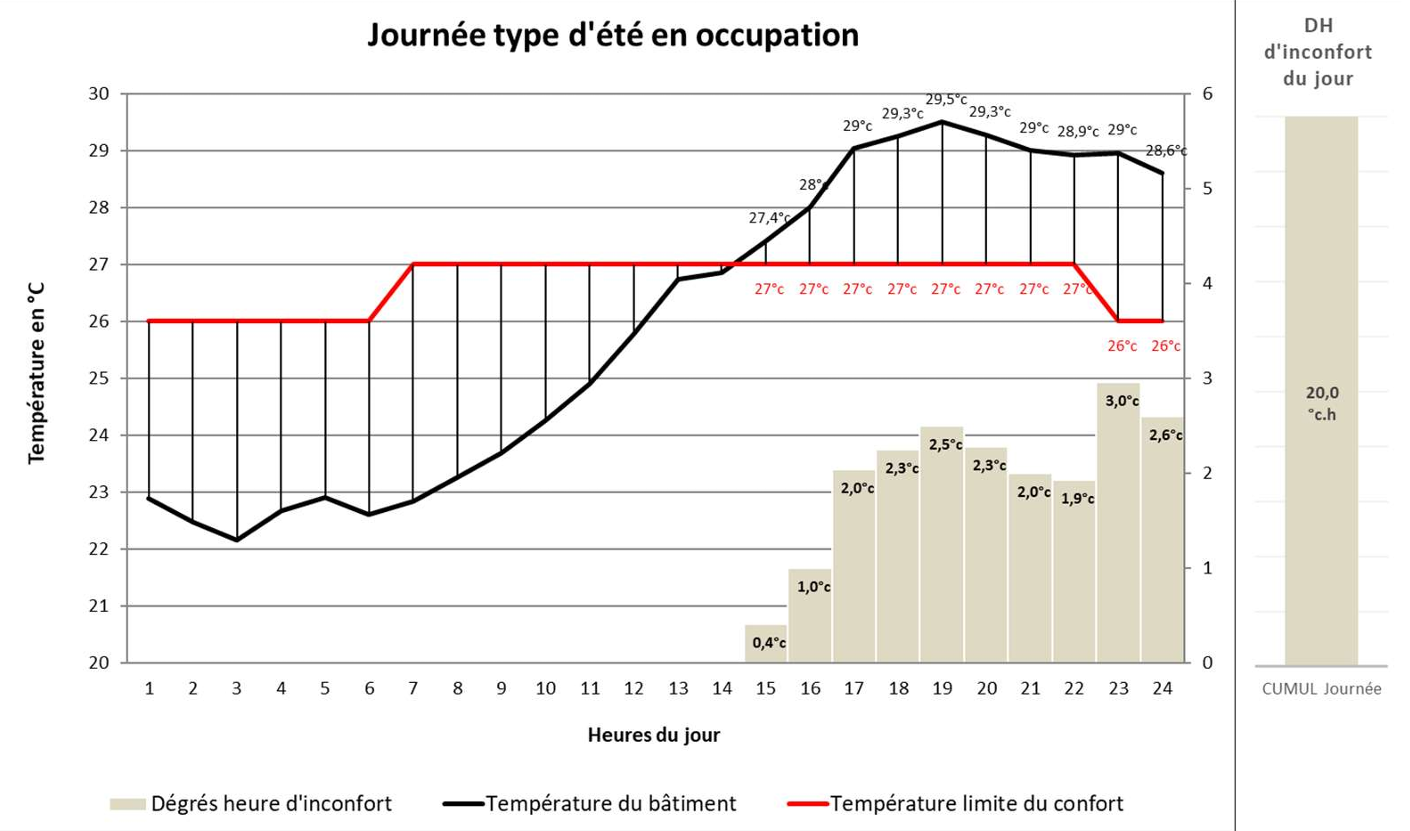
\includegraphics[width=0.5\linewidth]{figures/DH.png}
    \caption{Degrés-heures issus du Guide de la RE 2020 \footfullcite{guide-re2020}}
    \label{fig:dh}
\end{figure}

\section{Conclusion sur la RE 2020}
La RE 2020 est la réglementation environnementale en vigueur pour les projets neufs, elle se compose de 6 indicateurs qui doivent respecter les seuils (évolutifs). Ces 6 indicateurs sont regroupés en trois catégories : carbone, énergie et confort d'été, comme illustré sur le schéma~\ref{fig:20}.

\begin{figure}
    \centering
    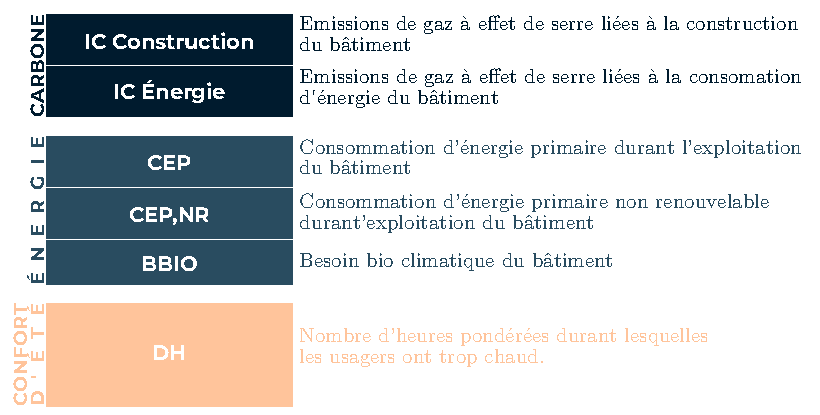
\includegraphics[width=1\linewidth]{figures/re.pdf}
    \caption{Synthèse des indicateurs de la RE 2020}
    \label{fig:20}
\end{figure}

\chapter{Conclusion sur le contexte}
